\section[pbdR]{pbdR: programming with big data in R}

\hidenum
\begin{frame}[noframenumbering]
\frametitle{Contents}
 \tableofcontents[currentsection,hideallsubsections]
\end{frame}
\shownum

\subsection{pbdR}

\begin{frame}
  \begin{block}{Programming with Big Data in R (pbdR)}
       \centering \emph{Productivity, Portability, Performance}\\[.4cm]
  \begin{columns}[onlytextwidth]
    \begin{column}{0.30\textwidth}
      \centering
       
\includegraphics[width=3.4cm]{../common/pics/simple}\\[.2cm]
    \end{column}
    \begin{column}{0.65\textwidth}
  \begin{itemize}
    \item \emph{Free}\footnote{MPL, BSD, and GPL licensed} R packages.
    \item Bridging high-performance C with high-productivity of R
    \item Distributed data details implicitly managed.
    \item Methods have syntax \emph{identical} to R.
  \end{itemize}
    \end{column}
​  \end{columns}
\end{block}
\end{frame}

\begin{frame}
  \begin{block}{pbdR Packages}
    \begin{center}
      \begin{columns}
        \begin{column}{.52\textwidth}
      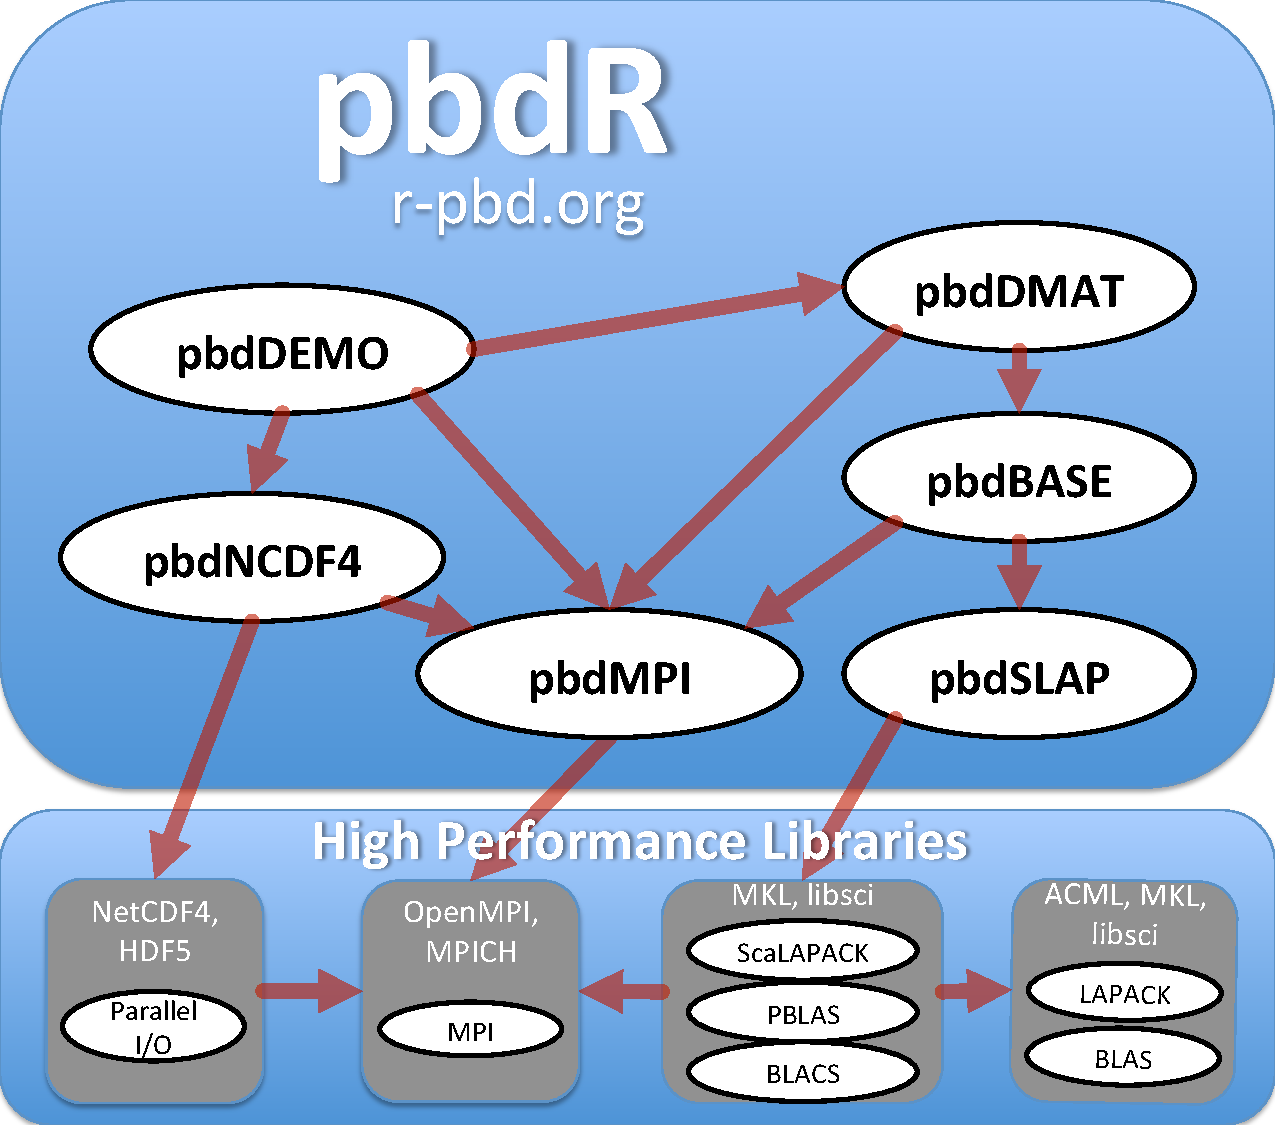
\includegraphics[scale=.3]{../common/pics/pbdR-graph}
        \end{column}
        \hfill
        \begin{column}{.4\textwidth}
      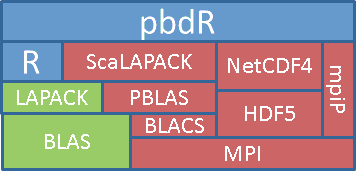
\includegraphics[scale=.45]{../common/pics/libs}
        \end{column}
      \end{columns}
    \end{center}
  \end{block}
\end{frame}

\begin{frame}
  \begin{block}{pbdR on HPC Resources}
    pbdR is currently installed and maintained on:
    \begin{itemize}
      \item Nautilus, UTK
      \item Kraken, UTK
      \item Newton, UTK
      \item Lens, ORNL
%       \item Titan, ORNL
      \item tara, UMBC
    \end{itemize}
    If you are interested in maintaining pbdR, contact us at 
\url{RBigData@gmail.com}
  \end{block}
\end{frame}

\begin{frame}[fragile]
  \begin{block}{pbdR Example Syntax}
  \begin{lstlisting}
x <- x[-1, 2:5]
x <- log(abs(x) + 1)
xtx <- t(x) %*% x
ans <- svd(solve(xtx))
  \end{lstlisting}
  \begin{center}
  Look familiar?\\[.4cm]
  \emph{It runs on 1 core with R or on 10,000 cores with pbdR}

%   \vspace{1em}
%   \emph{It also runs on 2 cores or 4 cores of your laptop with pbdR}
  \end{center}
  \end{block}
\end{frame}

\subsection{pbdR Paradigms}

\begin{frame}
  \begin{block}{pbdR Paradigms}
  Programs that use pbdR utilize:
  \begin{itemize}[<+-|alert@+>]
   \item Batch execution
   \item Single Program/Multiple Data (SPMD) style
%    \item Object Oriented Programming (OOP)
   \\[.2cm]
   \end{itemize}
    And generally utilize:
   \begin{itemize}
   \item Data Parallelism
  \end{itemize}
  \end{block}
\end{frame}


\begin{frame}[fragile]
  \begin{block}{Batch Execution}\pause
    \begin{itemize}
      \item Non-interactive
      \item Use
\vspace{-.4cm}
\begin{lstlisting}[language=sh]
Rscript my_script.r
\end{lstlisting}
or\vspace{-.4cm}
\begin{lstlisting}[language=sh]
R CMD BATCH my_script.r
\end{lstlisting}
      \item In parallel:
\vspace{-.4cm}
\begin{lstlisting}[language=sh]
mpirun -np 2 Rscript my_par_script.r
\end{lstlisting}
    \end{itemize}
  \end{block}
\end{frame}

\begin{frame}
  \begin{block}{Single Program/Multiple Data (SPMD)}\pause
    \begin{itemize}
      \item Difficult to describe, easy to do\dots
      \item Only one program is written, executed in batch on all processors.
      \item Different processors are autonomous; there is no manager.
      \item The dominant programming model for large machines.
    \end{itemize}
  \end{block}
  \begin{center}
    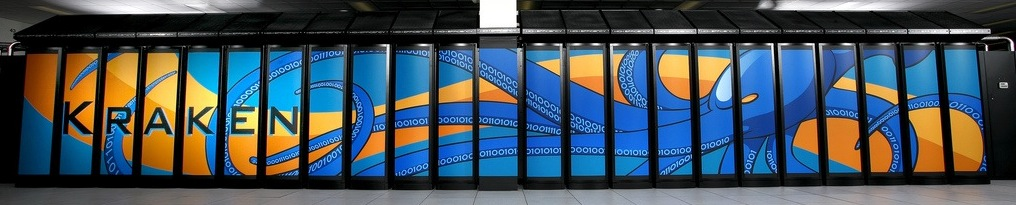
\includegraphics[width=11cm]{../common/pics/kraken1wide.jpg} \\
    Kraken: 112,896 cores in 9,408 nodes with 147 TB Memory
    \end{center}
\end{frame}

